\section{$PSF$ approximation for distributed deconvolution} \label{gradients}
For a distributed deconvolution, we would like to deconvolve the image with as little communication as possible. This largely depends on the size of the $PSF$ when compared to the overall image. If the $PSF$ is for example $\frac{1}{16}$ of the total image size, we have patches of the image which are completely independent of each other. Sadly, this is not true for radio interferometers. The $PSF$ is generally the same size as the image. We cannot deconvolve any part of the image independently of each other.

However, we have two effects of modern radio interferometers, that produce an "approximately" smaller $PSF$: First, we have an increasing number of visibilities. They create a $PSF$ that increasingly resembles a Gaussian function in the center, and the rest approaches zero. And secondly, we reconstruct images with a wide field-of-view. Although the $PSF$ is not zero the further away we move from the center, its values approach zero.

\begin{figure}[h]
	\centering
	\begin{subfigure}[b]{0.3\linewidth}
		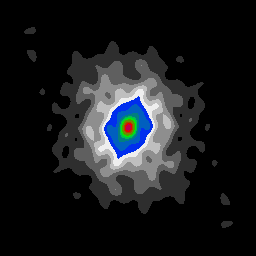
\includegraphics[width=\linewidth]{./chapters/03.distribution/simulated/psf.png}
	\end{subfigure}
	\begin{subfigure}[b]{0.3\linewidth}
		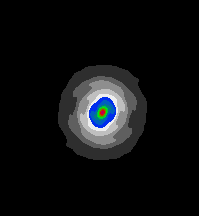
\includegraphics[width=\linewidth]{./chapters/06.gradient/psf_cut.png}
	\end{subfigure}
	
	\caption{$PSF$ arising from an increasing number of visibilities.}
\end{figure} 

In short, with an ever increasing number of visibilities and field-of-view, the influence of far-away image sections become negligible. We can approximate the deconvolution with a fraction of the true $PSF$. To our knowledge, we are the first to propose such approximation methods. In this Section, we present our approximation methods. In Section \ref{results:gradients}, we empirically demonstrate the validity of our approximations on a real-world MeerKAT observation. In Section \ref{pcdm}, we show more sophisticated coordinate descent methods that can exploit the smaller $PSF$. 

\subsection{Intuition for approximating the $PSF$}
Our basic coordinate descent algorithm chooses a pixel to minimize, calculates its gradient and descends in that direction. The gradient calculation reduces itself to a correlation of the residuals with the $PSF$ at the pixel location. In other words, we need the $PSF$ to calculate a gradient. If we only use parts of the $PSF$ for the calculation, we essentially approximate the gradient for the pixel. Because the $PSF$ only has significant non-zero values in the center, we should be able to ignore most of the values and still have an adequate gradient approximation.

Furthermore, our basic coordinate descent algorithm reconstructs inside the Major/Minor cycle framework. The framework is designed to handle only an approximate $PSF$ in the deconvolution (Remember: the $w$-term changes the $PSF$ depending on the position in the image). The framework may be able to deal with further $PSF$ approximations, namely with a $PSF$ that is reduced in size, which makes the distributed deconvolution simpler.

Indeed, this is the case, as we will demonstrate empirically in Section \ref{results:gradients}. But an approximation of the $PSF$ may lead to other problems in the reconstruction:
\begin{itemize}
	\item Needs additional Major cycles to converge.
	\item Slow down convergence speed of coordinate descent.
	\item Not guaranteed to converge to the same image.
\end{itemize}

The Major cycle corrects the errors the approximate $PSF$ introduces. The more inaccurate the $PSF$ is, the more Major cycles we may need to converge. As we already discussed, a Major cycle is an expensive operation. Our $PSF$ approximation should lead to as few (if any) additional Major cycles.

For the basic coordinate descent algorithm, an approximate $PSF$ may slow down the convergence speed. In each iteration, the basic algorithm finds the optimal value for the current pixel. With an approximate $PSF$, we may need several iterations on the same pixel (over several major cycles) until we arrive at the same value. In short, an approximate $PSF$ can slow down the convergence speed of coordinate descent.

Depending on how we approximate the $PSF$, we may not have any guarantee that we arrive at the same result. We developed two approximation methods: Method 1 uses an approximation in the gradient update step of coordinate descent. Method 2 solves an approximate deconvolution problem with only a fraction of the $PSF$. Only method 1 is guaranteed to converge to the same solution (with enough major cycles), but is slower to converge than method 2.

Depending on the method we use, we can remedy some of the problems that approximating the $PSF$ introduces. But there seems to be a trade-off to be made. We have not found a method that works best in every aspect.

\subsection{Method 1: Approximate gradient update}
The basic coordinate descent method first correlates the residuals with the $PSF$. It pre-calculates the gradient for each pixel. Then, in each iteration, it directly updates the map of gradients with the product of $PSF \star PSF$ (the $PSF$ correlated with itself). In this approximation method, we start from the same pre-calculated map of gradients, but use an approximate update. The first coordinate descent iteration of this approximation method is identical to coordinate descent with the full $PSF$. With each coordinate descent iterations, the gradient map becomes more inaccurate. But with enough major cycles, this method converges to the same result as when the full $PSF$ is used.

The question is, how do we approximate the product of $PSF \star PSF$. As we have seen before, the product of $PSF \star PSF$ also approaches zero away from the center (an example was shown in Figure \ref{cd:efficient:update:figure} in Section \ref{cd:efficient:update}). A naive way to approximate the update step is to "cut off" the insignificant value and only use a rectangle of the center, which is a fraction of the total image size. For example: An image of size $1024^2$ also has a $PSF$ the size of $1024^2$. The product $PSF \star PSF$ actually has the size of $2048^2$ pixels due to the correlation. We can try to approximate the product by only using the center rectangle $\frac{1}{8}$ of the total size, ($256^2$ pixels). This approximation works, but leads to artifacts during deconvolution: The image will be reconstructed in visible "blocks" which are the size of the center fraction we use. 

We chose another way. We approximate the product $PSF \star PSF$ as shown in equation \eqref{gradient:method1:psf2}, where $cut()$ is the function that cuts away everything but the center rectangle of the $PSF$. This is a better approximation than cutting the product directly, and leads to faster convergence.

\begin{equation}\label{gradient:method1:psf2}
PSF \star PSF \approx cut(PSF) \star cut(PSF)
\end{equation}

The reason why \eqref{gradient:method1:psf2} is a better approximation lies in the reason why we update the gradients with the product of $PSF \star PSF$ in the first place: It is the combination of two separate operations, removing the $PSF$ from the residuals at the current position, and recalculating the correlation with the $PSF$. If we cut away parts of the product $PSF \star PSF$ directly, we implicitly update the residuals with a different $PSF$. But when we approximate the product by \eqref{gradient:method1:psf2}, we ensure that the implicit removal of the $PSF$ from the residuals is equal to $cut(PSF)$.

In our implementation, we use one more trick to improve the approximation: we scale the product of $cut(PSF) \star cut(PSF)$ to have the same maximum as the original product $PSF \star PSF$.

Guaranteed to converge to the same result.
shows the $PSF$ and the corresponding productThis product too has 




So we use the full $PSF$

only update with a fraction of the $PSF$

$PSF$ squared update. Scaling.
So we become less and less accurate


\subsection{Method 2:Approximate deconvolution}

We never use the full PSF

But the problem of gradient magnitude. 

Change lambda. We do an approximate deconvolution. 


\subsection{Major Cycle convergence}\label{gradients:pathreg}

Sidelobe.

\cite{clark1980efficient} and the question on how many iterations per major cycle
Putting it all together

We have the Minor Cycle, which is easy to converge.

Coordinate Descent Path optimization \cite{friedman2010regularization}
Danger that CD takes too many pixel into a Major Cycle. Lower bound per iteration, PSF sidelobe
can still be too low, danger when many psf sidelobes overlap